\documentclass[12pt,a4paper]{article}
\usepackage[utf8]{inputenc}
\usepackage{amsmath}
\usepackage{amsfonts}
\usepackage{amssymb}
\usepackage{graphicx}
\usepackage{float}
\usepackage[table, svgnames, dvipsnames]{xcolor}
\usepackage{booktabs}
\usepackage{graphicx}
\usepackage{float}
\usepackage{ subcaption }
\usepackage{algorithm}
\usepackage{algorithmic}
\graphicspath{ {images/} }
\author{Alessio Ragno}
\title{Reinforcement Learning Project Report}
\date{November 2019}

\begin{document}

% \maketitle

\begin{titlepage}
    \begin{center}
        \vspace*{1cm}
        
        \huge
        \textbf{Reinforcement Learning Implementation Project Report}
        
        
        \vspace{1.5cm}
        \LARGE
        Alessio Ragno
        
        \vfill
        
        
\includegraphics[width=0.2\textwidth]{sapienza_logo.png}


        
        \vfill
        
  

        \vspace{0.5cm}
        
        
        \large
        Master's Degree in Artificial Intelligence and Robotics\break\break
        Department of Computer, Control and Management Engineering\break\break
        Sapienza University of Rome\break\break
        December 2019

    \end{center}
\end{titlepage}



\pagebreak
\tableofcontents
\pagebreak

\section{Introduction}

\section{Additional Tests and Conclusions}

\begin{figure}[H]
    \centering
    \begin{subfigure}[a]{0.4\textwidth}
        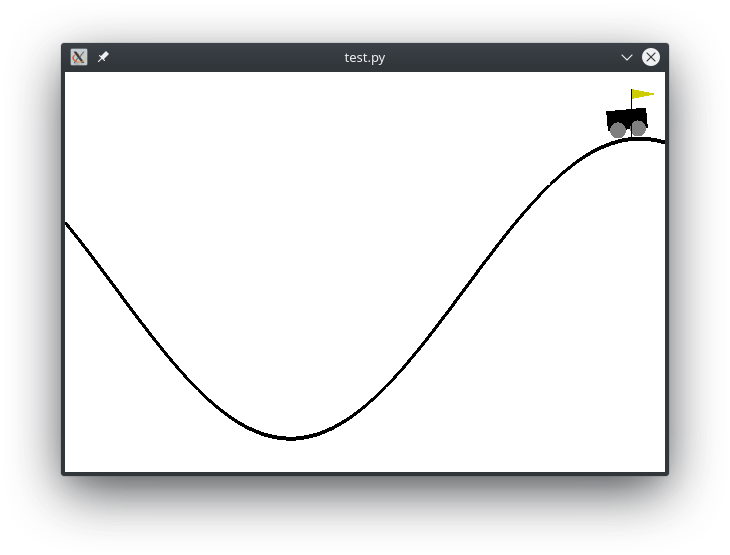
\includegraphics[width=\textwidth]{MountainCar-Victory}
        \caption{MountainCar-v0}
    \end{subfigure}
    \begin{subfigure}[a]{0.4\textwidth}
        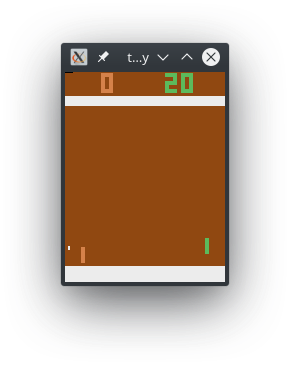
\includegraphics[width=\textwidth]{Pong-Victory}
        \caption{Pong-v4}
    \end{subfigure}
    \caption{Environments}
\end{figure}

What follows is the report for the Reinforcement Learning Implementation Project of Machine Learning Class of Master-s Degree in Artificial Intelligence and Robotics.

The project consists in the implementation of an assigned Reinfocement Learning algorithm and its evaluation in two different environments.

The assigned algorithm is Trust Region Policy Optimization (TRPO) and it has to be evaluated on the following OpenAI Gym environments:
\begin{itemize}
    \item \textbf{MountainCar-v0} is an environment in which a car has to climb a hill and reach a specific point indicated by a flag. MountainCar-v0 is a continuous state space environment that can be controlled with discrete actions. At each timestep the agent can choose between three actions: pushing the car left, right or not applying any force to the car.
    \item \textbf{Pong-v4} is an environment in which the agent has to play Pong game against a virtual player. The state is the image of the game and the agent acts using the Atari 2600 commands: NOOP, FIRE, RIGHT, LEFT, RIGHTFIRE, LEFTFIRE. For this project Pong-v4 has been used instead of Pong-v0 since the former is deterministic.
\end{itemize}

\section{Trust Region Policy Optimization}

Trust Region Policy Optimization was published by John Schulman, Sergey Levine, Philipp Moritz, Michael I. Jordan and Pieter Abbeel on April 2017. 
TRPO is an improvement of the vanilla Policy Gradient algorithm implemented by REINFORCE with baseline. TRPO aims to make gradient step which are not "too big" to improve the algorithm stability. The length of the step is defined in terms of a hyperparameter $\delta$ which represents the radius of the trust region.

\begin{algorithm}[H]
    \caption{TRPO}
\begin{algorithmic}[1]
\FOR{iteration = $1$,$2$,...}
    \STATE Run policy for $T$ timesteps or $N$ trajectories
    \STATE Estimate advantage function at all timesteps
    \FOR{$t = 1$, $T$}
        \STATE maximize $\sum_{n=1}^N \frac{\pi_\theta(a_n|s_n)}{\pi_{\theta_{old}}(a_n|s_n)} A_n$
        \STATE s.t. $\overline{KL}_{\pi_{\theta_{old}}}(\pi_\theta) < \delta$
    \ENDFOR
\ENDFOR
\end{algorithmic}
\label{alg:TRPO}
\end{algorithm}

\begin{algorithm}[H]
    \caption{TRPO}
\begin{algorithmic}[1]
\STATE Input: initial policy parameters $\theta_0$, initial value function parameters $\phi_0$
\STATE Hyperparameters: KL-divergence limit $\delta$, backtracking coefficient $\alpha$, maximum number of backtracking steps $K$
\FOR{$k = 0$,$1$,$2$, ...}
    \STATE Collect set of trakectories $D_k = \{\tau_i\}$ by running policy $\pi_k = \pi(\theta_k)$ in the environment
    \STATE Compute rewards-to-go $R_t$
    \STATE Compute advantage estimates, $A_t$ (using any method of advantage estimation) based on the current value function $V_{\phi_k}$
    \STATE Estimate policy gradient as
    $$ g_k = \frac{1}{D_k} \sum_{\tau \in D_k} \sum_{t=0}^T \nabla_{\theta} log \pi_\theta(a_t|s_t)|_{\theta_k} A_t$$
    \STATE Use the conjugate gradient algorithm to compute
    $$x_k = H^{-1}_k g_k$$
    where $H_k$ is the Hessian of the sample average KL-divergence
    \STATE Update the policy by backtracking line search with
    $$\theta_{k+1} = \theta_k + \alpha^j \sqrt{\frac{2\delta}{x_k^T H_kx_k}}x_k$$
    where $j \in \{0,1,2,...,K\}$ is the smallest value which improves the sample oss and satisfies the sample KL-divergence constraint
    \STATE Fit the value function by regression on mean-squared-error:
    $$\phi_{k+1} = arg min_\phi \frac{1}{|D_k|T}\sum_{\tau \in D_k} \sum_{t=0}(V_\phi(s_t) - R_t)^2$$
    tipically via some gradient descent algorithm
\ENDFOR
\end{algorithmic}
\label{alg:TRPO2}
\end{algorithm}

Algorithm \ref{alg:TRPO} shows the basic TRPO idea in pseudocode: It actually consists in a Vanilla Policy Gradient with the constraint of taking only "improving" steps.

To implement TRPO, the authors suggest to maximize the vanilla policy gradient (which they call surrogate loss) and at the same time minimize the KL divergence calculating the hessian vector product with the surrogate loss gradient.

After generating the step direction using conjugate gradients, the algorithm uses linesearch to find the right stepsize.

Applying the suggested calculation we obtain Algorithm \ref{alg:TRPO2}.

In the paper, the authors showed the hyperparameters used in each environment and it turned out that using $K=10$ maximum backtracking steps for the line search is sufficient.

Increasing $\delta$ the algorithm becomes more "aggressive" and at the same time unstable, while decreasing it, the algorithm learns slower but it is more cautious. The authors showed that using $\delta=0.01$ is a good tradeoff between velocity and stability.

Since the calculation of the gradients, the conjugate gradient and the linesearch make this algorithm computationally expensive, a more efficient and improved version was later published as Proximal Policy Optimization (PPO) by Schulman et al..

\section{Model Training and Evaluation}
 
This section shows the results obtained in the two environment mentioned above. For MountainCar-v0 using a fully connected was sufficient while for Pong-v0, which gives an image as observation, some tricks were necessary.

The code was fully written in Tensorflow 2.0 using Keras APIs for the construction of the Neural Networks. In Tensorflow 2.0, contrary to Tensorflow 1.x, eager execution is enabled by default and the graph is not kept for the whole execution but only built when needed. This led to multiple nested functions for the calculation of the gradients.

\subsection{MountainCar-v0}

\begin{figure}[H]
    \centering
    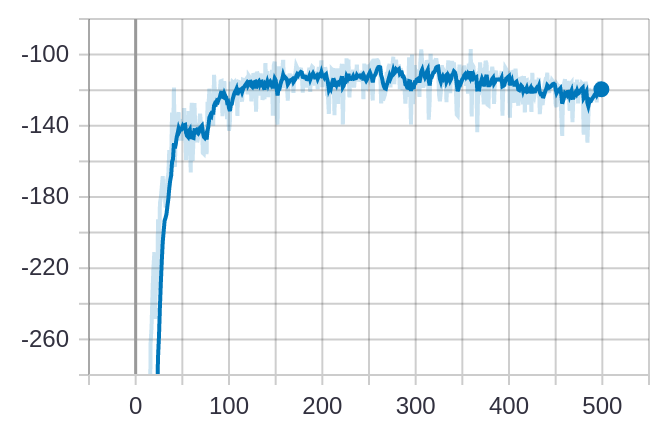
\includegraphics[width=0.5\textwidth]{MountainCar-v0.png}
    \caption{MountainCar-v0}
    \label{fig:MountainCar-v0}
\end{figure}

In MountainCar, a car has to climb a hill and reach a goal point taking advantage of the cumulated momentum. At each non-goal step, the agent is given a reward equal to -1 while when the goal is reached the episode is ended. The observation consists in the current position and velocity of the car.

The gym environment by default sets the maximum number of timesteps to 200. This turned out to be too low since the agent was not capable to reach the goal "randomly" within 200 steps. To ensure proper exploration the limit has been then increased to 1600.

Although this trick helped a little, the agent wasn't still capable of reaching the goal state enough times to learn a good policy. To solve this problem a "correlated $\epsilon$-greedy" algorithm for exploration was added to the policy: With probability $\epsilon$ the agent picks a random action, which is, with probability 0.8 the same of the last action. This increased a lot exploration, since, mostly in this environment, it is very likely that the best action to take at the next step is the same of the just taken one.

The agent was trained for 340 episodes and it converged to a mean total reward of -110 (it takes about 110 steps to reach the goal state). 

Figure \ref{fig:MountainCar-v0} is the plot of the mean total reward over the different training epochs.

It is possible to test this environment using the saved model \textit{"saved\_models/MountainCar\-v0/340.ckpt"} with the script "test.py". Also intermediate models have been saved.


\subsection{Pong-v4}

\begin{figure}[H]
    \centering
    \begin{subfigure}[b]{0.3\textwidth}
        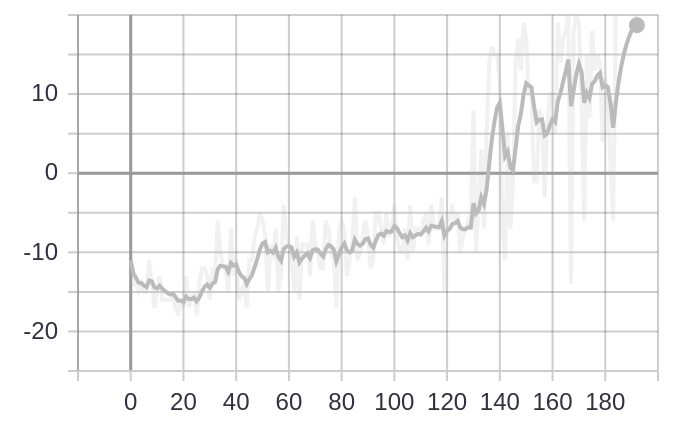
\includegraphics[width=\textwidth]{Pong-v4.png}
        \caption{Pong-v4}
        \label{fig:Max Reward}
    \end{subfigure}
    \begin{subfigure}[b]{0.3\textwidth}
        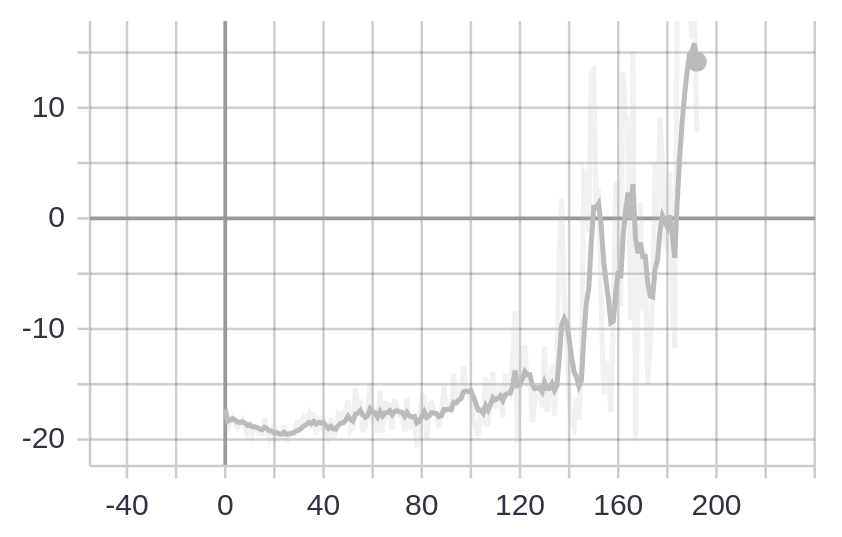
\includegraphics[width=\textwidth]{Pong-v4_mean.png}
        \caption{Pong-v4}
        \label{fig:Mean Reward}
    \end{subfigure}
    \caption{Pong-v4}
    \label{fig:Pong-v4}

\end{figure}

In Pong, the agent has to play Pong game using a simulated Atari 2600 console. The observation consists in the image perceived by the agent while the reward is the difference between the agent score and the opponent one.

The paper reports that for training Atari environments it took about 30hrs for them. Since a gpu wasn't available, the observation needed to be preprocessed. To make the learning process not too long, the agent was given as observation 3 integers which represent the position of the ball in the image and the height of the agent's stick. This preprocessing speeded up not only the training phase but also the sampling one. Not only the state space was reduced, but also the action one: not all the actions are necessary, so I decided to limit the action space to RIGHT and LEFT.

Moreover, to train Atari environments, the authors suggest to use vine sampling which consists in saving a state and performing different actions starting from the same state. This is unfortunally impossible to apply on all environments since it requires restoring a previous state and it is also very computationally expensive.

Altough reducing the input space to 3 integers helped a lot, the exploration phase was still too long. I decided to give it a hand by applying the optimal policy instead of a random one with $\epsilon$-greedy. This helped a lot, the algorithm was not only able to see a lot of space but it also learnt very quickly.

Figure \ref{fig:Pong-v4} is the plot of the mean total reward and the max reward over the different training epochs.
It is not possible to say that this environment has been solved since it doesn't actually reach a mean reward of 21, but given the complexity of the game and that the calculator architecture was probably not good as the authors one, these are quite good results.
It is possible to test this environment using the saved model \textit{"saved\_models/Pong-v4\-v0/340.ckpt"} with the script "test.py". Also intermediate models have been saved.


\section{Additional Tests and Conclusions}

\begin{figure}[H]
    \centering
    \begin{subfigure}[b]{0.3\textwidth}
        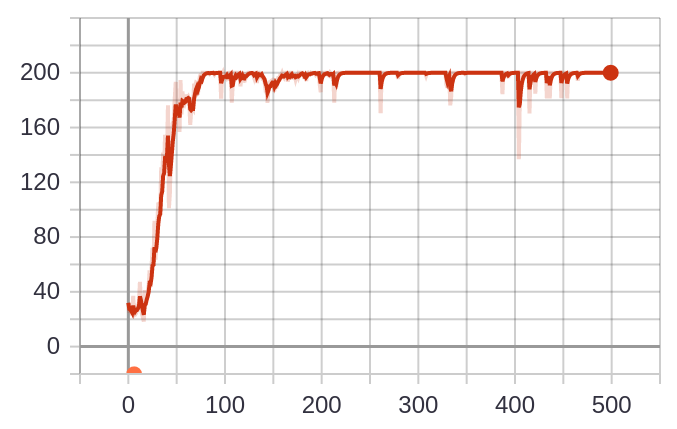
\includegraphics[width=\textwidth]{CartPole-v0.png}
        \caption{CartPole-v0}
        \label{fig:CartPole-v0}
    \end{subfigure}
    \begin{subfigure}[b]{0.3\textwidth}
        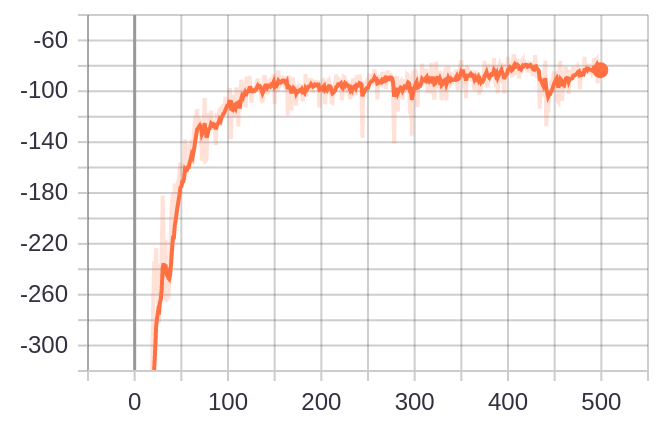
\includegraphics[width=\textwidth]{Acrobot-v1.png}
        \caption{Acrobot-v1}
        \label{fig:Acrobot-v1}
    \end{subfigure}
    \begin{subfigure}[b]{0.3\textwidth}
        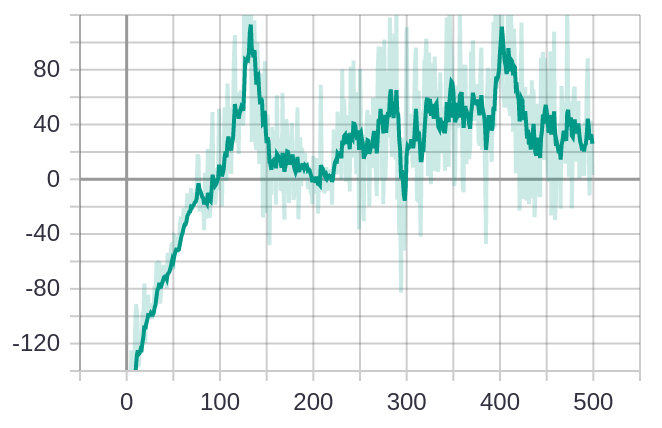
\includegraphics[width=\textwidth]{LunarLander-v2}
        \caption{LunarLander-v2}
        \label{fig:LunarLander-v2}
    \end{subfigure}
    \caption{Additional Environments}

    \label{fig:AdditionalEnvironments}

\end{figure}

Some additional tests have been run over different environments. In particular, three more environments have been tried out. Figure \ref{fig:AdditionalEnvironments} shows the reward plots of the training phases of CartPole-v0, Acrobot-v1 and LunarLander-v2. Also for these three environments pretrained models are given.
\end{document}


